\documentclass[12pt,utf8,notheorems,compress]{beamer}
\usepackage{etex}

\usepackage[english]{babel}

\usepackage{tikz}
\usetikzlibrary{decorations.pathmorphing,arrows}
\usepackage{mathtools}
\usepackage{booktabs}
\usepackage{ragged2e}
\usepackage{multicol}
\usepackage{tabto}
\usepackage{xstring}

\usepackage[protrusion=true,expansion=false]{microtype}

\setlength\parskip{\medskipamount}
\setlength\parindent{0pt}

\renewcommand{\U}{\mathcal{U}}
\newcommand{\NN}{\mathbb{N}}
\newcommand{\ZZ}{\mathbb{Z}}
\newcommand{\RR}{\mathbb{R}}
\newcommand{\Id}{\mathrm{Id}}
\newcommand{\fst}{\mathsf{fst}}
\newcommand{\snd}{\mathsf{snd}}
\newcommand{\refl}{\mathsf{refl}}
\renewcommand{\succ}{\mathsf{succ}}
\newcommand{\seg}{\mathsf{seg}}
\newcommand{\base}{\mathsf{base}}
\newcommand{\lloop}{\mathsf{loop}}
\newcommand{\surf}{\mathsf{surf}}
\newcommand{\merid}{\mathsf{merid}}
\newcommand{\N}{\mathsf{N}}
\renewcommand{\S}{\mathsf{S}}
\newcommand{\Cyl}{\mathrm{Cyl}}
\newcommand{\IsContr}{\mathsf{IsContr}}
\newcommand{\IsMereProp}{\mathsf{IsMereProp}}
\newcommand{\IsSet}{\mathsf{IsSet}}
\newcommand{\IsEquiv}{\mathsf{IsEquiv}}
\newcommand{\LEM}{\mathsf{LEM}}
\newcommand{\UIP}{\mathsf{UIP}}
\newcommand{\fib}{\mathsf{fib}}
\newcommand{\defeq}{\vcentcolon=}
\newcommand{\defeqv}{\vcentcolon\equiv}
\newcommand{\ct}{%
  \mathchoice{\mathbin{\raisebox{0.5ex}{$\displaystyle\centerdot$}}}%
             {\mathbin{\raisebox{0.5ex}{$\centerdot$}}}%
             {\mathbin{\raisebox{0.25ex}{$\scriptstyle\,\centerdot\,$}}}%
             {\mathbin{\raisebox{0.1ex}{$\scriptscriptstyle\,\centerdot\,$}}}
}

\title{Homotopy type theory}
\author[Arbeitsseminar Geometrie/Topologie]{\vspace{-1em}\\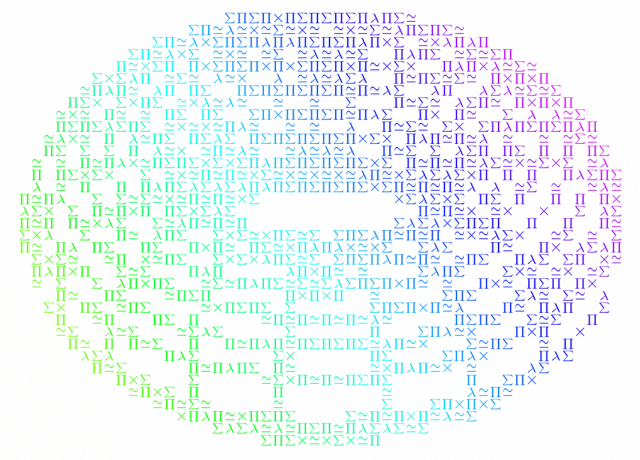
\includegraphics[scale=0.3]{torus.png} \\[0.5em] Ingo Blechschmidt \\[-0.3em] {\scriptsize November 25th, 2014}}
\date{November 25th, 2014}

\usetheme{Warsaw}
\definecolor{mypurple}{RGB}{200, 35, 180}
%\setbeamercolor{structure}{fg=purple}
\usecolortheme{seahorse}
%\usecolortheme{purple}?
%\usefonttheme{default}?
%\usepackage{kurier}?
\usefonttheme{serif}
%\usepackage{libertine}?
\usepackage{mathpazo}
\useinnertheme{rectangles}

\setbeamertemplate{frametitle}[default][colsep=-2bp,rounded=false,shadow=false,center]

\setbeamertemplate{headline}{}
\setbeamertemplate{navigation symbols}{}

\newcommand{\floatbox}[3]{%
  \raisebox{0pt}[0pt][0pt]{%
    \begin{picture}(0,0)(#1,#2)#3\end{picture}\leavevmode%
  }%
}

\newcommand{\backupstart}{
  \newcounter{framenumberpreappendix}
  \setcounter{framenumberpreappendix}{\value{framenumber}}
}
\newcommand{\backupend}{
  \addtocounter{framenumberpreappendix}{-\value{framenumber}}
  \addtocounter{framenumber}{\value{framenumberpreappendix}} 
}

\newcommand*\oldmacro{}%
\let\oldmacro\insertshorttitle%
\renewcommand*\insertshorttitle{%
  \oldmacro\hfill\insertframenumber\,/\,\inserttotalframenumber\hfill}

\newcommand{\hil}[1]{{\usebeamercolor[fg]{item}{\textbf{#1}}}}

\newcommand{\img}[3]{\begin{center}\includegraphics[scale=#1]{#2}\\\small#3\end{center}}
%\newcommand{\imageslide}[3]{\frame{\frametitle{#1}\img{#2}{#3}}}

\IfSubStr{\jobname}{\detokenize{nonotes}}{
  \setbeameroption{hide notes}
}{
  \setbeameroption{show notes}
}
\setbeamertemplate{note page}[plain]

\begin{document}

\frame{\titlepage}

\frame[t]{\frametitle{Outline}\scriptsize\begin{itemize}\item[]\tableofcontents\end{itemize}}

\note{\justifying\fontsize{8pt}{9.6}\selectfont
  \setlength{\columnsep}{1em}
  \begin{multicols}{2}
    Homotopy type theory is a new branch of mathematics that combines
    aspects of several different fields in a surprising way. It is part of
    Voevodsky's \emph{univalent foundations} program and based on a recently
    discovered connection between homotopy theory and type theory, a branch
    of mathematical logic and theoretical computer science.

    In homotopy type theory, any set (really: \emph{type}) behaves like a
    topological space, or more precisely, a homotopy type. The basic notion
    of equality is reimagined in an interesting way: Analogous to how two
    given points in a space may be joined by more than one path, two
    elements of a set can be equal in many ways. A new axiom, the
    \emph{univalence axiom}, posits that equivalent structures really are
    the same, thus formalizing a widespread notational practice.

    Besides explaining how working in homotopy type theory feels like, the
    talk will give answers to the listed questions.
    The talk does not assume any background in formal logic or type theory.
    \columnbreak

    \begin{itemize}
    \justifying
    \item What are logical foundations for mathematics and why should we care?
    \item What are the disadvantages of traditional set-based approaches to foundations?
    \item Why is the development of homotopy theory radically simplified in
    homotopy type theory?
    \item How are the seemingly diverse activities of \emph{proving
    propositions} and \emph{exhibiting constructions} identified?
    \item How do inductive definitions of important spaces concisely capture
    their homotopy-theoretic content?
    \item Why is homotopy type theory a major step towards practically useful
    and easily applicable proof assistants?
    \end{itemize}
  \end{multicols}
}


\section{Foundations}

\subsection{What are foundations?}

\frame[t]{\frametitle{What are foundations?}
  \begin{itemize}
    \item Foundations set the logical context for doing maths.
    \item Their details don't matter in everyday work (mostly).
    \item But their main concepts do.
  \end{itemize}

  \only<1>{\img{0.25}{bridge}{\tiny\url{http://collabcubed.com/2012/10/24/high-trestle-trail-bridge-rdg/}}}
  \only<2>{\begin{itemize}
    \item Classical foundations are \emph{set-based} (ZF, ZFC, \ldots):
          \hil{Everything is a set.}
    \item $0 \defeq \emptyset$, \quad
          $1 \defeq \{0\}$, \quad
          $2 \defeq \{0,1\}$, \quad
          $\ldots$
    \item $(x,y) \defeq \{ \{x\}, \{x,y\} \}$ \quad (Kuratowski pairing)
    \item $(x,y,z) \defeq (x,(y,z))$
    \item maps: $(X,Y,R)$ with $R \subseteq X \times Y$ such that \ldots
  \end{itemize}}
}

\note{
  \begin{itemize}
    \item Foundations allow us to be maximally precise.
    \item A \emph{proof} as commonly understood is really a shorthand for a
    (never spelled out) fully formal proof.
    \item Unlike informal proofs, the correctness of a formal proof can be
    checked mechanically.
  \end{itemize}

  \img{0.5}{logicomix}{Logicomix: An Epic Search for Truth}
}


\subsection{What's problematic with set-based foundations?}

\frame[t]{\frametitle{What's wrong with set-based foundations?}
  Set-based foundations \ldots
  \begin{itemize}
    \item do not reflect typed mathematical practice,
    \item do not respect equivalence of structures,
    \item require complex encoding of ``higher-level'' subjects,
          complicating interactive proof environments.
  \end{itemize}
}

\note{
  \begin{itemize}
    \item Examples for questions which can be formulated:
    \begin{itemize}
      \item Is $2 = (0,0)$? (No, when using my definitions.)
      \item Is $\sin \in \pi$? (Depends on your definitions.)
    \end{itemize}
    \item\justifying In ordinary practice, these questions would be deemed as nonsensical,
    since they disrespect the \emph{types} of mathematical objects and are not
    invariant under isomorphisms of the involved structures.
    \item Note: There are also \emph{structural approaches} to set theory
    without a global membership predicate (e.\,g.\@ ETCS), resolving this
    defect.
  \end{itemize}
}

\note{
  \begin{itemize}
    \item\justifying Fully unravel the definition of ``manifold'' in set-theoretical
    language to get a grasp of the complex encodings needed.
    \item This is no problem for humans, but it is for machines.
    \item Voevodsky: ``The roadblock that prevented generations of interested
    mathematicians and computer scientists from solving the problem of computer
    verification of mathematical reasoning was the unpreparedness of
    foundations of mathematics for the requirements of this task.''
  \end{itemize}

  \begin{itemize}
    \item Note: Set theory is perfectly fine for studying \emph{sets}.
  \end{itemize}
}


% Now the fun begins! :-)
\setbeamercolor{structure}{fg=purple}

\section{Basics on homotopy type theory (HoTT)}

\subsection{What is homotopy type theory?}

\frame[t]{\frametitle{What is homotopy type theory?}
  \begin{itemize}
    \item Homotopy type theory is a new foundational theory.
    \item Basic notions have a homotopy-theoretic flavour.
    \item One can start doing ``real mathematics'' right away, without complex encodings.
    \item Initiated by Voevodsky in 2005.
  \end{itemize}

  \img{0.2}{authors}{Some participants of the IAS special year}
}

\frame[t,label=awesome]{\frametitle{What is homotopy type theory?}
  Homotopy type theory \ldots
  \begin{itemize}
    \item is elegant,
    \item reflects mathematical practice,
    \item contains wondrous new concepts,
    \item ensures that everything respects equivalences,
    \item simplifies the plumbing of homotopy theory,
    \item allows for accessible computer formalization.
  \end{itemize}

  \transfade<2>[duration=40]
  \visible<2>{\img{0.1}{awesome}{}}
  % http://1.bp.blogspot.com/-cPQyFx7EvCc/UxVEm6Td29I/AAAAAAAAfBg/HZ1AwI2re9Q/s1600/unikitty.png
}

\note{
  \begin{itemize}
    \item\justifying Homotopy type theory is approximately \emph{intensional Martin-Löf type
    theory} (existing since the 1970s) plus the new \emph{univalence axiom}.
    \item After repeatedly experiencing mistakes in his field going unnoticed
    for several years, Voevodsky wanted to work with proof assistants. He went
    public in 2009.
    \item Voevodsky: ``This story got me scared. Starting from 1993 multiple groups of
    mathematicians studied the [\ldots] paper at seminars and used it in their
    work and none of them noticed the mistake.

    And it clearly was not an accident. A technical argument by a trusted author, which 
    is hard to check and looks similar to arguments known to be correct, is
    hardly ever checked in detail.''
  \end{itemize}
}

\note{
  Results which have been fully formalized in HoTT include:
  \begin{itemize}
    \item $\pi_1(S^1)$
    \item $\pi_{k \leq n}(S^n)$
    \item $\pi_{n+1}(S^n)$ is cyclic for all $n \geq 3$
    \item fiber sequences and the long exact sequence
    \item the Hopf fibration
    \item the Freudenthal suspension theorem
    \item the van Kempen theorem
    \item the Blakers--Massey theorem
  \end{itemize}
}


\subsection{What are values and types?}

\frame[t]{\frametitle{What are values and types?}
  \begin{itemize}
    \item In type theory, there are \hil{values} and \hil{types}.
    \item Every value is of exactly one type.
    \item Types may depend on values.
  \end{itemize}
  \begin{align*}
    7 &: \NN \\
    (3,5) &: \NN \times \NN \\
    \succ &: \NN \to \NN \\
    \text{zero vector} &: \RR^n \quad\text{($n : \NN$)}
  \end{align*}

  \visible<2>{
  Let~$B(x)$ be a type family depending on $x:A$.
  \begin{itemize}
    \item $\sum_{x:A} B(x) = \text{``$\{ (a,b) \,|\, a:A, b:B(a) \}$''}$
    \item $\prod_{x:A} B(x) = \text{``$\{ f : A \to {??} \,|\, \text{$f(a) : B(a)$ for
    all $a:A$} \}$''}$
  \end{itemize}}
  \floatbox{-250}{-90}{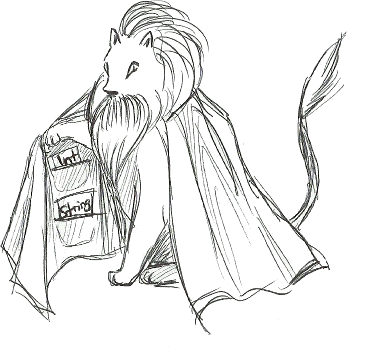
\includegraphics[scale=0.7]{martin-loef}}
}

\note{
  \begin{itemize}
    \item\justifying Types are familiar from programming (\texttt{Int},
    \texttt{String}, \ldots).
    \item But the type systems of well-known mainstream languages are either
    trivial (Ruby, Python: everything is an object) or not very expressive (C,
    Java).
    \item Haskell and languages of the ML family have a rich type system,
    encompassing function types and algebraic data types.
    \item But even their type systems do not support \emph{dependent types} --
    types which may depend on values. Look to Coq or Agda for those.
  \end{itemize}
}

\note{
  In the special case that~$B(x) \defeqv B$ does not depend on $x$:
  \[ \sum_{x:A} B \equiv A \times B \qquad
    \prod_{x:A} B \equiv (A \to B) \]
}


\subsection{What is the dependent equality type?}

\frame[t]{\frametitle{What is the dependent equality type?}
  In set theory, for a set~$X$ and elements~$x,y \in X$:
  \begin{itemize}
    \item ``$x=y$'' is a \hil{proposition}.
    \item Set theory is \hil{layered above} predicate logic.
  \end{itemize}
  \bigskip

  In type theory, for a type~$X$ and values~$x,y : X$:
  \begin{itemize}
    \item There is the \hil{equality type} $\Id_X(x,y)$ or $(x =_X y)$.
    \item To verify that ``$x=y$'',
    exhibit a value of~$(x = y)$.
    \item Have $\refl_x : (x = x)$.
    \item Identity types may contain zero or \hil{many} values!
  \end{itemize}
  Intuition: $(x = y)$ is the type of \hil{proofs} that ``$x=y$''.

  \pause
  Intuition: $(x = y)$ is the type of \hil{paths} $x \leadsto y$.
}

\note{
  \begin{itemize}
    \item\justifying Note that we use logical terminology. A proposition is merely a
    statement, not necessarily a true statement.
    \item In an intensional type theory, propositions are not an extra part of
    the language, distinct from values and types.
    \item Instead, \emph{propositions are types}.
    \item To prove a proposition means to exhibit a value of it.
    Such a value can be thought of as a \emph{proof} or \emph{witness}.
    \item We have \emph{proof relevance}.
    \item Types which values are all equal -- types for which merely knowing that they
    are inhabited -- are called \emph{mere propositions}. See below for
    $\IsMereProp$.
  \end{itemize}
}

\note{
  Examples for more complex propositions (types):
  \begin{itemize}
    \item ``$X$ is a subsingleton'': \tabto{4.9cm}
    $\prod_{x:X} \prod_{y:X} (x=y)$
    \item ``Addition is commutative'': \tabto{4.9cm}
    $\prod_{n:\NN} \prod_{m:\NN} (n+m = m+n)$
    \item ``Every number is even'': \tabto{4.9cm}
    $\prod_{n:\NN} \sum_{m:\NN} (n=2m)$
  \end{itemize}
}


\section{Homotopy theory in HoTT}

\subsection{How are types like spaces?}

\frame[t]{\frametitle{How are types like spaces?}
  \begin{center}\begin{tabular}{ll}
    \toprule
    homotopy theory & type theory \\\midrule
    \hil{space} $X$ & type $X$ \\
    \hil{point} $x \in X$ & value $x:X$ \\
    \hil{path} $x \leadsto y$ & value of $(x = y)$ \\
    \hil{(continuous) map} & value of $X \to Y$ \\
    \bottomrule
  \end{tabular}\end{center}

  \begin{itemize}
    \item A \hil{homotopy} between maps $f, g : X \to Y$ is a value of
    \[ (f \simeq g) \defeqv \prod_{x:X} (f(x) = g(x)). \]
    \item A space $X$ is \hil{contractible} iff
    \[ \IsContr(X) \defeqv \sum_{x:X} \prod_{y:X} (x=y). \]
  \end{itemize}
}

\frame[t]{\frametitle{How are types like spaces?}
  \begin{itemize}
  \item ``The type $X$ is \hil{contractible}'':
    \[ \IsContr(X) \defeqv \sum_{x:X} \prod_{y:X} (x=y). \]

  \item ``The type $X$ is a \hil{mere proposition}'':
  \[ \IsMereProp(X) \defeqv \prod_{x,y:X} (x = y) \]

  \item ``The type $X$ is a \hil{set} or \hil{discrete space}'':
  \[ \IsSet(X) \defeqv \prod_{x,y:X} \IsMereProp(x = y) \]

  \item For instance, $\NN$ is a set.
  \end{itemize}
}

\frame[t]{\frametitle{How are types like spaces?}
  \begin{itemize}
    \item Functions are automatically \hil{continuous/functorial}:
    \[ (x = y) \longrightarrow (f(x) = f(y)). \]

    \item Type families $P : X \to \U$ automatically behave like
    \hil{fibrations}, in that they have the path lifting property:
    \[ (x = y) \longrightarrow (P(x) \simeq P(y)). \]
  \end{itemize}
}


\subsection{How are constructions encoded?}

\frame[t]{\frametitle{How are constructions encoded?}
  \begin{itemize}
    \item The \hil{fiber} of a map $f : X \to Y$ over a point $y:Y$ is
    \[ \fib_f(y) \defeqv \sum_{x:X} (f(x) = y). \]

    \item The \hil{path space} of $X$ is
    \[ X^I \defeqv \sum_{x,y:X} (x=y). \]

    \item The \hil{based loop space} of $X$ at $x$ is
    \[ \Omega^1(X,x) \defeqv (x=x). \]

    \item The \hil{path fibration} of $(X,x)$ is the map
    \[ \snd : \sum_{y:X} (x=y) \to X. \]
  \end{itemize}
  \floatbox{-250}{-45}{\only<2>{
\includegraphics[scale=0.5]{look-ma}}}
}

\note{
  For doing homotopy theory in HoTT, the following are \emph{not} needed:
  \begin{itemize}
    \item open sets
    \item construction of topologies on equivalence classes of paths
    \item real numbers
    \item axiom of choice
    \item law of excluded middle
    \item \ldots
  \end{itemize}
}


\subsection{What are higher inductive definitions?}

\frame[t]{\frametitle{What are higher inductive definitions?}
  The type~$\NN$ of natural numbers is \hil{freely generated} by
  \begin{itemize}
    \item a point $0 : \NN$ and
    \item a function $\succ : \NN \to \NN$.
  \end{itemize}
  This definition gives rise to an \hil{induction principle}
  \[ \prod_{A:\NN \to \U}
    \Bigl(
    A(0) \times \Bigl(\prod_{n:\NN} A(n) \to A(\succ(n))\Bigr) \longrightarrow
    \prod_{n:\NN} A(n)
    \Bigr), \]
  and a \hil{recursion principle}
  \[ \prod_{X:\U}
    \Bigl(
    X \times \Bigl(\NN \to (X \to X)\Bigr) \longrightarrow
    (\NN \to X)
    \Bigr). \]
}

\note{
  \begin{itemize}
    \item\justifying $\U$ is a \emph{universe}. Its values are types.
    \item The recursion principle is the specialization of the induction
    principle to constant type families $A(n) \equiv X$.
    \item In a \emph{higher} inductive definition, constructors may not only
    generate \emph{points}, but also \emph{paths} and \emph{higher paths}. 
    \item We will drop the adjective ``freely''.
  \end{itemize}
}

\frame[t]{\frametitle{How to present famous spaces?}
%  The \hil{interval} $I$ is generated by
%  \begin{itemize}
%    \item a point $0 : I$ and
%    \item a point $1 : I$ and
%    \item a path $\seg : (0 = 1)$.
%  \end{itemize}
%  Of course, we can show $I \simeq \boldsymbol{1}$.
%  \bigskip
%  \pause

  The \hil{circle} $S^1$ is generated by
  \begin{itemize}
    \item a point $\base : S^1$ and
    \item a path $\lloop : (\base = \base)$.
  \end{itemize}
  \bigskip

  The \hil{sphere} $S^2$ is generated by
  \begin{itemize}
    \item a point $\base : S^2$ and
    \item a path $\surf : (\refl_\base = \refl_\base)$.
  \end{itemize}
  \bigskip

  The \hil{torus} $T^2$ is generated by
  \begin{itemize}
    \item a point $b : T^2$,
    \item a path $p : (b = b)$,
    \item a path $q : (b = b)$, and
    \item a 2-path $t : (p \ct q = q \ct p)$.
  \end{itemize}
}

\note{
  \begin{itemize}
    \item\justifying Note that a presentation of a type \emph{determines}, but does not
    \emph{explicitly describe} its higher identity types.
    \item Just like the free vector space spanned by set contains not only the
    given elements, but also their linear combinations, the type given by a
    higher inductive definition (or its higher identity types) may contain many
    more values than explicitly listed.
    \item For instance, there is a nontrivial element in $(\refl_{\refl_\base}
    = \refl_{\refl_\base})$, where $\base : S^2$, corresponding to the
    \emph{Hopf fibration}.
    \item Also, different generators may turn out to give rise to the same
    element.
  \end{itemize}
}

\frame[t]{\frametitle{How to present famous spaces?}
  The \hil{suspension} $\Sigma X$ of $X$ is generated by
  \begin{itemize}
    \item a point $\N : \Sigma X$ and
    \item a point $\S : \Sigma X$ and
    \item a function $\merid : X \to (N = S)$.
  \end{itemize}
  \bigskip

  The \hil{cylinder} $\Cyl(X)$ of $X$ is generated by
  \begin{itemize}
    \item a function $\mathsf{bot} : X \to \Cyl(X)$ and
    \item a function $\mathsf{top} : X \to \Cyl(X)$ and
    \item a function $\seg : \prod_{x:X} (\mathsf{bot}(x) = \mathsf{top}(x))$.
  \end{itemize}
  Of course, we can show $\Cyl(X) \simeq X \times I \simeq X$.
}


\subsection{What is circle induction?}

\frame[t]{\frametitle{What is circle induction?}
  \setlength{\columnsep}{-1.5em}

  % Stolen from HoTT/hits.tex, of course.
  \begin{center}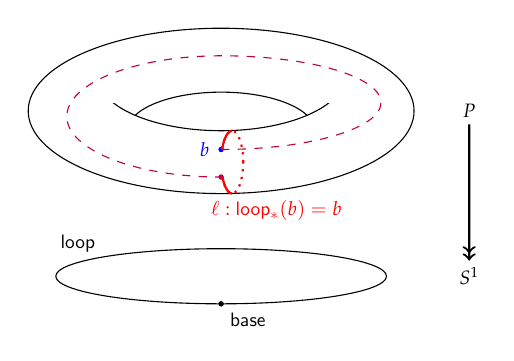
\begin{tikzpicture}[scale=0.7, transform shape]
    \draw (0,0) ellipse (3 and .5);
    \draw (0,3) ellipse (3.5 and 1.5);
    \begin{scope}[yshift=4]
      \clip (-3,3) -- (-1.8,3) -- (-1.8,3.7) -- (1.8,3.7) -- (1.8,3) -- (3,3) -- (3,0) -- (-3,0) -- cycle;
      \draw[clip] (0,3.5) ellipse (2.25 and 1);
      \draw (0,2.5) ellipse (1.7 and .7);
    \end{scope}
    \node (P) at (4.5,3) {$P$};
    \node (S1) at (4.5,0) {$S^1$};
    \draw[->>,thick] (P) -- (S1);
    \node[fill,circle,inner sep=1pt,label={below right:$\base$}] at (0,-.5) {};
    \node at (-2.6,.6) {$\lloop$};
    \node[fill,circle,blue,inner sep=1pt] (b) at (0,2.3) {};
      \node[blue] at (-.3,2.3) {$b$};
      \node[fill,circle,purple,inner sep=1pt] (tb) at (0,1.8) {};
      % \draw[\OPTpurple,dashed] (b) to[out=0,in=0,looseness=5] (0,4) to[out=180,in=180] (tb);
      \draw[purple,dashed] (b) arc (-90:90:2.9 and 0.85) arc (90:270:2.8 and 1.1);
      \begin{scope}
        \clip (b) -- ++(.1,0) -- (.1,1.8) -- ++(-.2,0) -- ++(0,-1) -- ++(3,2) -- ++(-3,0) -- (-.1,2.3) -- cycle;
        \draw[red,dotted,thick] (.2,2.07) ellipse (.2 and .57);
        \begin{scope}
          % \draw[clip] (b) -- ++(.1,0) |- (tb) -- ++(-.2,0) -- ++(0,-1) -| ++(3,3) -| (b);
          \clip (.2,0) rectangle (-2,3);
          \draw[red,thick] (.2,2.07) ellipse (.2 and .57);
        \end{scope}
      \end{scope}
      \node[red] at (1,1.2) {$\ell: \lloop_*(b)=b$};
  \end{tikzpicture}\end{center}

  The \hil{induction principle} of $S^1$ states: Given $P : S^1 \to \U,$
  \begin{multicols}{2}
  \begin{itemize}
    \item a point $b : P(\base)$, and
    \columnbreak
    \item a path $\ell : \lloop_*(b) = b$
  \end{itemize}
  \end{multicols}
  there is a function $f : \prod_{x:S^1} P(x)$ such that
  \begin{multicols}{2}
  \begin{itemize}
    \item $f(\base) \equiv b$ and
    \columnbreak
    \item $f(\lloop) = \ell$.
  \end{itemize}
  \end{multicols}
}

\note{
  \begin{itemize}
    \item\justifying In particular, restricting to constant type families, we
    obtain the recursion principle of $S^1$. It says that functions $S^1 \to X$
    are given by a point $b : X$ and a loop $(b = b)$.
  \end{itemize}
}


\section{Further topics}

\subsection{What is type truncation?}

\frame[t]{\frametitle{What is type truncation?}
  Let $X$ be a type.

  The \hil{propositional truncation} $\|X\|_{-1}$ is generated by
  \begin{itemize}
    \item a function $X \to \|X\|_{-1}$ and
    \item for any $x, y : \|X\|_{-1}$, a path $x = y$.
  \end{itemize}
  \bigskip

  The \hil{0-truncation} $\|X\|_0$ is generated by
  \begin{itemize}
    \item a function $X \to \|X\|_0$ and
    \item for any $x, y : \|X\|_0$, $p, q : (x = y)$, a path $p = q$.
  \end{itemize}
  \bigskip

  The \hil{fundamental group} of $(X,x_0)$ is
  \[ \pi_1(X,x_0) \defeqv \| \Omega^1(X,x_0) \|_0 \defeqv \| (x_0 = x_0) \|_0. \]
}

\note{
  \begin{itemize}
    \item\justifying Similarly, one can define the \emph{$n$-truncation} of a type for
    any $n \geq -2$.
    \item $\|X\|_{-1}$ is a mere proposition, $\|X\|_0$ is a set (discrete space).
    \item More generally and precisely, $\|X\|_n$ is the reflection of $X$ in
    the world of $n$-types, i.\,e.\@ its $n$-th \emph{Postnikov section}.
    \item $\|X\|_0$ is the set of connected components of $X$.
  \end{itemize}

  \begin{itemize}
    \item\justifying By circle induction, an equivalent definition is
    \[ \pi_1(X,x_0) \defeqv \| (S^1,\base) \to (X,x_0) \|_0, \]
    i.\,e.\@ the set of connected components of the space of
    base\-point-preserving functions $S^1 \to X$.
  \end{itemize}
}


\subsection{What is the univalence axiom?}

\frame[t]{\frametitle{What is the univalence axiom?}
  An \hil{equivalence} is a function $f : X \to Y$ such that
  \[ \IsEquiv(f) \defeqv \prod_{y:Y} \IsContr(\fib_f(y)). \]
  \medskip

  Types $X$ and $Y$ are \hil{equivalent} iff
  \[ (X \simeq Y) \defeqv \sum_{f : X \to Y} \IsEquiv(f). \]
  \medskip

  The \hil{univalence axiom} states: The canonical function
  \[ (X = Y) \longrightarrow (X \simeq Y) \]
  is an equivalence, for all types $X$ and $Y$.
}

\note{
  \begin{itemize}
    \item\justifying By the univalence axioms, equivalent types \emph{really are} equal.
    \item It implies that isomorphic groups, vector spaces, \ldots\@ are equal.
    \item Thus the widespread practice of \emph{pretending} that isomorphic
    structures are equal is rigorously formalized.
    \item The univalence axiom guarantees that \emph{any construction respects
    equivalence}.
    \item Most results require the univalence axiom.
  \end{itemize}
}

\note{
  \begin{itemize}
    \item\justifying The univalence axiom implies \emph{function
    extensionality}: The canonically defined function
    \[ (f = g) \longrightarrow \prod_{x:A} (f(x) = g(x)) \]
    is an equivalence, for all functions $f,g : A \to B$.
    \item So homotopic functions are equal.
  \end{itemize}
}

\note{
  \begin{itemize}
    \item\justifying Without the univalence axiom, it is consistent to assume
    \emph{uniqueness of identity proofs}, i.\,e.\@
    \[ \UIP \defeqv \prod_{X:\U} \prod_{x,y:X} \prod_{p,q:(x=y)} (p=q), \]
    thus collapsing the homotopical universe.
    \item Phrased differently, the univalence axiom can not be added to an
    \emph{extensional} type theory (one fulfillung $\UIP$).
  \end{itemize}

  \begin{itemize}
    \item\justifying \emph{No computational interpretation of the univalence axiom is
    known yet.} This prevents us from \emph{running} proofs (as computer
    programs). See below.
  \end{itemize}
}


\subsection{What's the status of the axiom of choice?}

\frame[t]{\frametitle{What's the status of the axiom of choice?}
  \begin{itemize}
    \item The following proposition is \hil{just true},
    but is not a faithful rendition of the axiom of choice:
    \[ \Bigl(\prod_{x:A} \sum_{y:B} R(x,y)\Bigr) \longrightarrow
    \sum_{f : A \to B} \prod_{x:A} R(x,f(x)). \]
    \item The real axiom of choice,
    \[ \Bigl(\prod_{x:A} \Bigl\|\sum_{y:B} R(x,y)\Bigr\|_{-1}\Bigr) \longrightarrow
    \Bigl\|\sum_{f : A \to B} \prod_{x:A} R(x,f(x))\Bigr\|_{-1}, \]
    can be added as an axiom, but is rarely needed.

    \pause
    \item The law of excluded middle is too rarely needed.
    \[ \LEM \defeqv \prod_{A:\U} \Bigl(\IsMereProp(A) \to A + \neg A\Bigr). \]
  \end{itemize}
}

\note{
  \begin{itemize}
    \item\justifying When doing homotopy theory in a classical set-based
    setting, one has to sometimes use the law of excluded middle or even the
    axiom of choice. This is an \emph{artifact} of the chosen encoding in set
    theory. It is \emph{not} due to an inherent unconstructivity of homotopy
    theory.

    \item Also recall that even in set-based mathematics, the law of excluded
    middle and the axiom of choice are not needed as often as it might first
    appear.

    \item Adding these two axioms prevents us from running proofs. In contrast
    to the univalence axiom, where it is believed that a computational
    interpretation might be found, this is less clear with these classical
    axioms.
  \end{itemize}
}

\note{
  \begin{itemize}
    \item Since the law of excluded middle as stated refers only to mere
    propositions ($(-1)$-types), it is also denoted ``$\LEM_{-1}$''.
    \item A law of excluded middle may not refer to \emph{all} types,
    i.\,e.\@
    \[ \LEM_\infty \defeqv \prod_{A:\U} \Bigl(A + \neg A\Bigr), \]
    is inconsistent with the univalence axiom.
  \end{itemize}
}


\subsection{What are models of HoTT?}

\frame[t]{\frametitle{What are models of HoTT?}
  Conjecturally, HoTT can be interpreted in any \hil{$\boldsymbol{(\infty,1)}$-topos}. Verified
  models include
  \begin{itemize}
    \item ${\infty}\mathrm{Grpd}$, i.\,e.\@ a model in simplicial sets, and
    \item $(\infty,1)$-presheaf toposes over elegant Reedy categories.
  \end{itemize}

  Thus, any theorem proven in HoTT holds in the context of classical homotopy
  theory and in more general contexts.
}

\note{
  The prototypical $(\infty,1)$-topos ${\infty}\mathrm{Grpd} \simeq
  \mathrm{Top}[\mathrm{whe}^{-1}] \simeq \mathrm{Kan}$ is equivalently:
  \begin{itemize}
    \item\justifying the $(\infty,1)$-category of all $(\infty,1)$-groupoids,
    \item the localization of the category of topological spaces (which have
    the homotopy type of a CW complex) at the class of weak homotopy
    equivalences, and
    \item the category of Kan complexes.
  \end{itemize}
}


\backupstart

\againframe{awesome}

\section{References}

\frame[t]{\frametitle{References}
  \begin{itemize}
    \item The textbook

    {\tiny\url{http://homotopytypetheory.org/book/}\par}

    \item Voevodsky on his motivations

    {\tiny
    \url{http://www.math.ias.edu/~vladimir/Site3/Univalent_Foundations_files/2014_IAS.pdf}\par}

    \item Seminar slides

    {\tiny
    \url{http://www.math.ias.edu/~mshulman/hottseminar2012/01intro.pdf}
    \url{http://www.math.ias.edu/~mshulman/hottminicourse2012/04induction.pdf}
    \url{https://coq.inria.fr/files/coq5-slides-spitters.pdf}
    \url{https://www.andrew.cmu.edu/user/awodey/hott/CMUslides.pdf}\par}

    \item An application unrelated to homotopy theory

    {\tiny\url{http://www.cs.nott.ac.uk/~txa/talks/lyon14.pdf}\par}

    \item hott-amateurs mailing list
  \end{itemize}
}

\backupend

\end{document}
